\chapter{Specifikacija rada}

Ovaj rad za cilj ima teoretski opisati i prakti\v{c}nim primjerom testirati dvija sli\v{c}na be�i\v{c}ne protokola, NFC (Near Field Communication) i BLE (Bluetooth Low Energy). Motivi za odabir ovakve teme uklju\v{c}uju relativnu , veliko podru\v{c}je primjene i razli\v{c}ite mogu\'{c} nosti koje pru�aju oba protokola. Me\dj utim, glavni motiv je sveprisutnost navedenih protokola jer danas gotovo svaki novi pametni telefon ima ugra\dj en NFC i BLE modul. Ako se uzme u obzir da je kori�tenje pametnog telefona postala svakodnevica gotovo polovice ljudi na svijetu (po izvje�\'{c} u ?Ericsson Mobility Report? tvrtke Ericsson \cite{mobilityReport} 2015. godine se u svijetu se koristilo 3,4 milijardi pametnih telefona, a predvi\dj eno je da \'{c} e se do 2021. ta brojka popeti do \v{c}ak 6,4 milijardi), dolazi se do zaklju\v{c}ka da mobilne aplikacije koje u svojim funkcionalnostima koriste NFC ili BLE protokol imaju potencijalno ogromno tr�i�te. Ipak, treba sa rezervom uzeti toliku brojku jer se oba protokola tek po\v{c}inju ugra\dj aviti u ve\'{c} inu novih pametnih telefona, dok su ih proteklih godina proizvo\dj a\v{c}i ugra\dj ivali samo u svoje najja\v{c}e i najskuplje modele.

Sli\v{c}nost protokola je u tome �to se oba koriste za be�i\v{c}nu komunikaciju kratkog dometa. Me\dj utim, tehnologija koja se koristi za implementaciju protokola je potpuno razli\v{c}ita. NFC za prijenos podataka koristi svojstva elektromagnetske indukcije, dok se kod BLE-a prijenos podataka ostvaruje preko radio valova. Samim time su svojstva protokola razli\v{c}ita (najbolji primjer je domet - NFC u praksi ima domet do 5 cm, a BLE do 10 metara) �to na kraju rezultira razli\v{c}itom primjenom u praksi. Upravo zato su protokoli komplementarni i zajedno se ugra\dj uju u pametne telefone jer zajedno mogu pru�iti rje�enje za gotovo sve potrebe u kratko dometnoj komunikaciji (razina prostorije). Naravno, razlog tome je i to �to su pametni telefon vrlo napredni ure\dj aji koji osim NFC i BLE modula imaju i GSM modul, modul za mobilni internet i WiFi modul, koji nisu uvijek optimalni za komunikaciju u kratkom dometu. Me\dj utim, kombinacija svih navedenih modula i mogu\'{c} nosti protokola koje implementiraju, \v{c}ini pametni telefon tako naprednim ure\dj ajem bez kojeg je �ivot modernog \v{c}ovjeka u 21. stolje\'{c}u nezamisliv.

Zbog svega navedenog, temeljna ideja ovog rada je implementirati oba protokola u sustav koji ima smisla i koji ima potencijala za�ivjeti na dana�njem tr�i�tu. Nastavak ovog poglavlja sadr�i opis sustava, aktivnosti koje su poduzete za ostvarivanje sustava te krajnji rezultat.

\section{Specifikacija sustava}

Glavna ideja sustava je kreirati mobilnu aplikaciju i administrativno su?elje koje bi trgova?ki lanci koristili za promociju proizvoda u svojim poslovnicama. Ideja je da trgova?ki lanaci preko web su?elja kreiraju popuste za svoje proizvode u odabranim poslovinicama, a zatim kupci pomo?u mobilne aplikacije ostvaruju kreirane popuste. Korisni?ko iskustvo je zami�ljeno tako da korisnik prilikom ulaza u poslovnicu, pomo?u pametnog telefona sa instaliranom aplikacijom te NFC i BLE modulom, skenira NFC naljepnicu koja aplikaciji daje informaciju u koju je poslovnicu korisnik u�ao. Mobilna aplikacija zatim dohva?a konfiguraciju te poslovnice poslovnice sa poslu�itelja, te je ta akcija je prikazana na slici ~\ref{fig:skeniranjeNaljepnice}.

\begin{figure}[!htbp]
	\begin{center}
 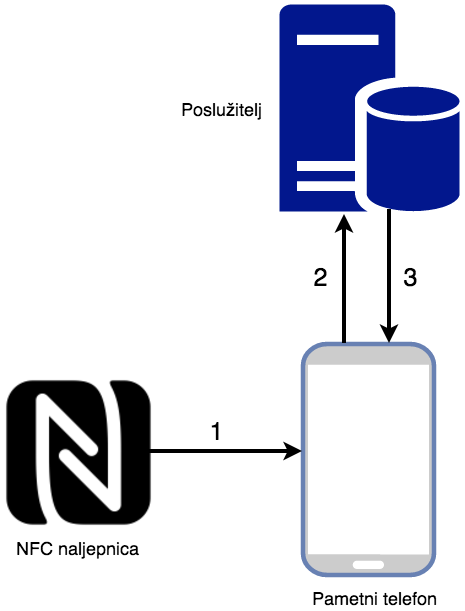
\includegraphics[height=12cm,keepaspectratio=true]{nfc_sken}
 \caption{Prikaz procesa skeniranja NFC nalijepnice (1), zahtjeva za konfiguracijom poslovnice (2) i dobivanje konfiguracje poslovnice (3).}
 \label{fig:skeniranjeNaljepnice}
	\end{center}
\end{figure}

Kada je aplikacija dobila konfiguraciju po?inje sa skeniranjem okoline, s ciljem nala�enja BLE ure?aja. Proizvodi na akciji imaju u svojoj neposrednoj blizini BLE ogla�iva? te korisniku koji prolazi pokraj police od proizvoda, ukoliko ima upaljenu aplikaciju, prona?eni popust postaje vidljiv u aplikaciji. Tada, ukoliko se odlu?i na iskori�tavanje popusta, kreira zahtjev za kodom popusta. Zahtjev je vezan za korisnikov ure?aj (zbog za�tite od zloupotrebe - svaki ure?aj mo�e jedan popust ostvariti maksimalno jedan put) te korisnik dobiva kod za popust kojeg je, s ciljem ostvarivanja popusta, du�an prikazati na blagajni. Opisani postupci su prikazani na slici  ~\ref{fig:otkrivanjeBLEa}.

\begin{figure}[!htbp]
	\begin{center}
 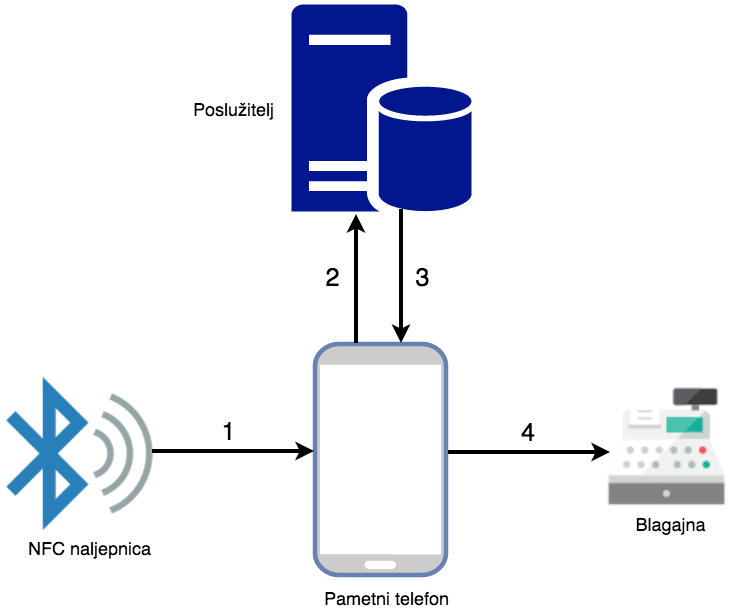
\includegraphics[height=12cm,keepaspectratio=true]{ble_sken}
 \caption{Prikaz procesa otkrivanja BLE ogla�iva?a (1), zahtjev za kodom skeniranog popusta (2), dobivanje koda za popust (3) i prikazivanje koda na blagajni za kona?no ostvarivanje popusta (4).}
 \label{fig:otkrivanjeBLEa}
	\end{center}
\end{figure}

Za implementaciju opisanog sustava potrebne su slijede?e aktivnosti:
\begin{enumerate}
	\item Kreiranje web aplikacije sa su?eljem za poslovne subjekte
	\item Kreiranje API su?elja za komunikaciju mobilne aplikacije i poslu�itelja
	\item Konfiguriranje NFC naljepnica i BLE ogla�iva?a
	\item Kreiranje mobilne aplikacije
	
\end{enumerate}

Resursi potrebni za ostvarivanje aktivnosti uklju?uju
\begin{enumerate}
	\item NFC naljepnice
	\item BLE ogla�iva?i
	\item Pametni telefon s integriranim NFC i BLE modulom
	\item Poslu�itelj za pohranjivanje web aplikacije i baze podataka
\end{enumerate}


\section{Rezultati}

Rezultat ovog rada je teoretska obrada dva sli?na be�i?na protokola za prijenos podataka te sustav koji objedinjuje i NFC i BLE protokol te uz pomo?u njihovih specifi?nosti korisnicima pru�a novo i druga?ije iskustvo u obavljanju kupovine. Prakti?ni dio rada uklju?uje u potpunosti funkcionalnu web i mobilnu aplikaciju. Web aplikacija se sastoji od dva dijela:

\begin{itemize}
	\item Su?elje za trgova?ke lance
	\begin{itemize}
		\item Implementirano dodavanje i ure?ivanje poslovnica
		\item Implementirano dodavanje popusta za odre?eni proizvod i povezivanje popusta sa odgovaraju?im ogla?iva?em
		\item Implementirano upravljanje popustima i pregledavanje iskori�tenih popusta
	\end{itemize}
	\item API su?elje
	
	\begin{itemize}
		\item Omogu?ava komunikaciju poslu�itelja i mobilne aplikacij
	\end{itemize}
\end{itemize}

Funkcionalnosti mobilne aplikacij uklju?uju:
\begin{enumerate}
	\item Skeniranje NFC naljepnica
	\item Tra�enje BLE ogla�iva?a u okolini
	\item Komunikacija sa poslu�iteljem
\end{enumerate}

U nastavku rada su opisane specifi?nosti NFC i BLE protokola, specifi?nosti tehnologija i alata pomo?u kojih je sustav kreiran, detaljan opis implementacije sustava te na poslijetku usporedba i evaluacija opisanih protokola.





